\chapter{Raw Tire Data}
\setcounter{figure}{0}
\setcounter{table}{0}

\label{sec:RawTireData}
The raw data item in the project tree contains the imported data and provides some tools for manipulating the data. These tools allow the data to be quickly and conveniently viewed and fitted to tire models.

The raw data form, shown in Figure~\ref{fig:RawTireDataForm}, is displayed when a raw data item in the project tree is clicked on. This form has a place to store comments about the test data contained in the item. It also contains the \textsl{Data Cropping} and \textsl{Data Collapsing} tools. The \textsl{Data Cropping} tool allows user to easily view and eradicate erroneous or undesired data from the raw data. The \textsl{Data Collapsing} tool removes hysteresis from the data and separates the data into sets depending on the conditions that the tire was tested at. Once the data has been collapsed a summary of the separated data sets will appear in the table in the raw data from. The \textsl{Model Fitting} tool in this section allows you to fit the raw or collapsed data to a tire model. Tire model fitting will be covered in more detail in section~\ref{sec:TireModels}.

The Options button at the top of the raw data form allows you to add another data file, export the tire data, or access the \textsl{Data Cropping} tool. A more detailed description of these operations is included in this section. The Data Comments allow the user to enter notes and information about the data. This information will be saved with the raw data in OptimumTire.

\begin{figure}[H]
	\centering
		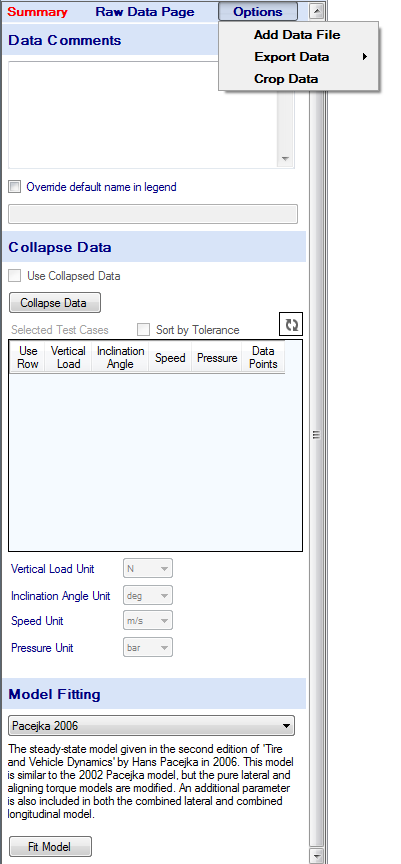
\includegraphics[height=0.95\textheight]{RawTireDataForm.png}
		\caption{Raw Tire Data Form Before Collapsing}
	\label{fig:RawTireDataForm}
\end{figure}

\section{Importing Data}
\label{sec:ImportingData}
When the \textsl{Add Raw Data} button above the project tree is clicked on, an open file window will appear. OptimumTire can open either a .rtd file, which is the OptimumTire binary format for tire data, or a CSV or ASCII file with .csv or .dat file extensions. Files with no extension are assumed to be CSV/ASCII files.

If a .rtd file is opened, the data will be automatically imported in the correct format and coordinate system. No further actions are required by the user.

If a CSV or ASCII file is selected a dialog box as shown in Figure~\ref{fig:ImportOptions} will open. In this box the the file properties can be specified. The character that separates the columns in the file and then the character that represents the decimal point should be selected. Multiple column separators can be selected if different file formats are to be used.

\begin{figure}[H]
	\centering
		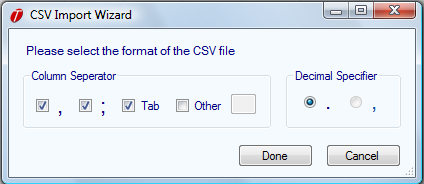
\includegraphics{ImportOptions.png}
	\caption{CSV Import Options}
	\label{fig:ImportOptions}
\end{figure}

If a CSV or ASCII file is opened, the data import wizard, shown in Figure~\ref{fig:DataImportWizard}, will appear. In this window the user specifies what quantity each column of raw data contains (i.e. SA, SR, Fx, etc) and the unit for that quantity. At the bottom of the dialog box, default values for quantities that are missing from the data can be specified. For example, if inflation pressure was not recorded in the test, the user could manually enter a constant inflation pressure to be included in the data. The coordinate system that the data was collected also needs to be specified.

\begin{figure}[H]
	\centering
		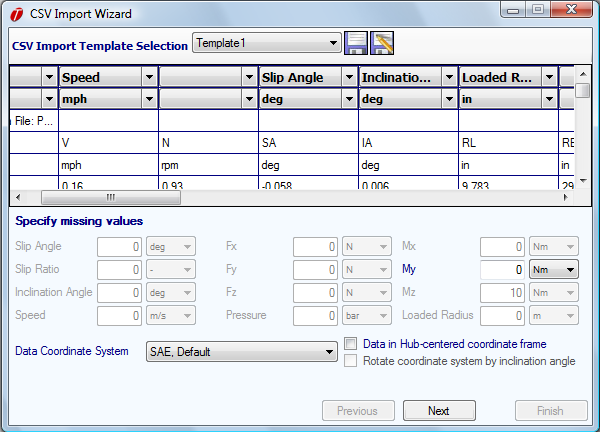
\includegraphics[width=1.0\textwidth]{DataImportWizard.png}
	\caption{Data Import Wizard}
	\label{fig:DataImportWizard}
\end{figure}

This process can be automated by using the import template feature at the top of Figure 2.1. The template to be used is chosen through the \textsl{CSV Import Template Selection} dropdown box. It can be seen in the figure that currently Template 1 is selected. New import templates can easily be created and saved. First the data quantities, units, and coordinate system are specified.  Then to save this as an import template, click the \textsl{Save as New Template} button. Import templates can also be modified and saved by using the \textsl{Save Template} button.

Typically tire data provides the force and moments at the center of the tire contact patch. However sometimes, especially with wheel force transducer data, it will be the force and moments at the wheel center. Therefore the \textit{Data in Hub-centered coordinate frame} checkbox should be selected. Then OptimumTire will transform the force and moment data to the center of the  contact patch. If this is the case the \textit{Rotate coordinate system by inclination angle} can also be selected. This should be done if the coordinate system that the force and moments were measured in are fixed to the wheel. In this case the vertical force would be in the same direction as the inclination angle and not perpendicular to the ground. Therefore if this option is selected OptimumTire will transform the forces and moments to a ground fixed coordinate system.

Once all of the column definitions have been assigned pressing the Next button will show a preview of the data to be imported. If the data to be imported is correct, clicking on Finish will import the data into OptimumTire.

Generally different sets of raw data should be imported into OptimumTire as separate files. However multiple test files can be imported and combined in OptimumTire. This can be achieved in two ways. If the files are in exactly the same format, simply select both files at the same time (use the shift or ctrl keys to choose more than one file). The import wizard will appear for the first file and the other files will be imported with exactly the same settings.

If the files are in different formate, multiple import into the same data item is done by importing the first data set as would normally be done. After this is completed, click on the data set in the project tree. Then select Add Data in the Options button in the upper right corner of the raw data form (see Figure \ref{fig:AddData}).  This will open the same CSV Import Wizard that was used previously. Follow the same steps as before and the data will be added to the previously imported set.

\begin{figure}
	\centering
		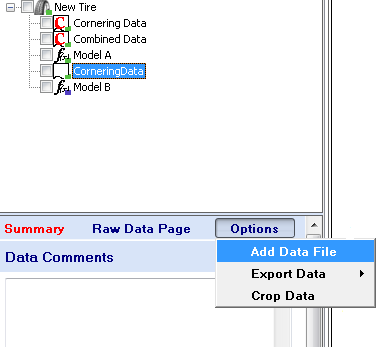
\includegraphics[width=0.50\textwidth]{AddData.png}
	\caption{Adding more data to a data set that has already been imported}
	\label{fig:AddData}
\end{figure}

\section{Importing TYDEX Data}
\label{sec:ImportingTYDEX Data}
Tire data stored in the TYDEX file format can be imported into OptimumTire. The process will load any TYDEX files the user specifies and will convert these into the CSV/ASCII format which is the default OptimumTire tire data format.

Click the \textsl{TYDEX} button in the \textsl{Add Raw Data} drop down menu to launch the TYDEX import wizard. In the window click \textsl{Add Files} to add in all the TYDEX files which should be imported. The TYDEX import will combine all the TYDEX files into a single OptimumTire tire data object which can be used for model fitting. Generally, select all TYDEX files from a single test run (multiple sweeps) in the add file dialog.

Once the files have been added they can be selected or un-selected using the checkboxes in the file list window. Un-selected files will not be included in the import process. By clicking on one of the files in the list, additional information from the TYDEX file is the displayed in the textbox. 

\begin{figure}[H]
	\centering
		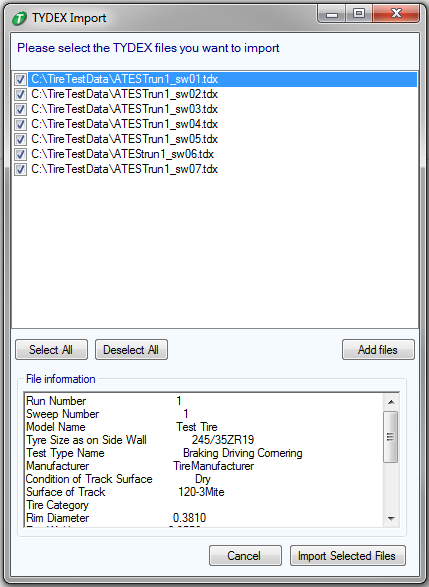
\includegraphics[width=0.5\textwidth]{TYDEXImport.png}
	\caption{TYDEX File Import Wizard}
	\label{fig:TYDEXImport}
\end{figure}

Clicking \textsl{Import Selected Files} converts the TYDEX files into a single CSV/ASCII files and the \textsl{Add Raw Data} import tool is automatically launched.

\section{Data Cropping}
\label{sec:DataCropping}
Data cropping allows the user to remove any unwanted or unnecessary data. Often in tire tests the data from conditioning or warm up procedures is included in the data file. This data can be easily removed in OptimumTire. 
The raw data can be cropped by selecting \textsl{Crop Data} under the \textsl{Options} button on the top of the raw data form. This will open the \textsl{Crop Data} window as shown in Figure~\ref{fig:DataCroppingTool}. The raw data to be cropped is displayed in the graph. You can select what properties of the raw data are graphed by selecting the checkboxes on the left. In the figure slip angle is represented by the blue line and the inclination angle by the red line. By clicking on the boxes to the right of the properties the color of the property can be changed. The values to the right of this correspond to the data values at the location of the black line on the graph. At the bottom the units of the data and the axis ranges can be changed. 

\begin{figure}[H]
	\centering
		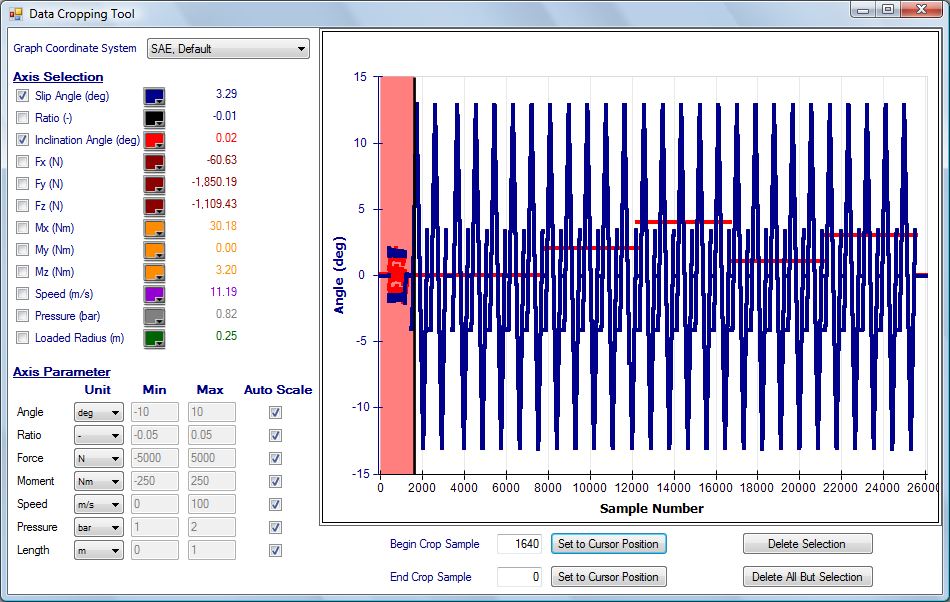
\includegraphics[width=1.0\textwidth]{DataCroppingTool.png}
	\caption{Data Cropping Tool}
	\label{fig:DataCroppingTool}
\end{figure}

As can be seen at the beginning and end of the run extra data exists that is not necessary. The data to be removed can be selected by entering the beginning and ending sample numbers in the \textsl{Begin Crop Sample} and \textsl{End Crop Sample} textboxes at the bottom of the window. Alternatively the vertical black line on the graph can be dragged to the point where the data should be cropped. Pressing the corresponding \textsl{Set} button defines the beginning or ending sample number. The background of the selected data will be pink. Then the \textsl{Delete Selection} or \textsl{Delete All But Selection} buttons can be clicked to remove the selected data. Figure \ref{fig:CroppedData} displays the data from Figure~\ref{fig:DataCroppingTool} after it has been cropped. As can be seen only the relevant test data remains. When the Crop Data is closed the program will return to the primary OptimumTire screen with cropped data.
 
 \begin{figure}[H]
	\centering
		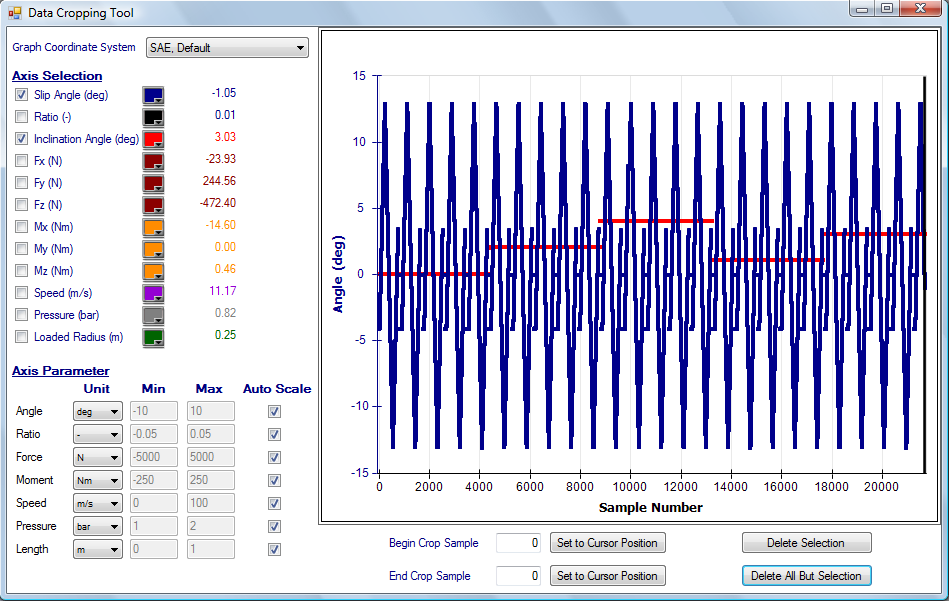
\includegraphics[width=1.0\textwidth]{CroppedData.png}
	\caption{Cropped Data}
	\label{fig:CroppedData}
\end{figure} 


\subsection{Data Cropping Templates}
\label{sec:DataCropping:templates}

To simplify the task of repetitively cropping data, templates can be set up. Crop templates record the beginning and ending sample number of each section deleted. The same actions can be applied to another data file. The file on which a template is used must be at least on long as the largest ending sample number in the template. A warning will be displayed if the crop template was created for a data file with a different number of samples than the one its being applied to. 

To record a crop template, simply crop a data file as usual. Once this is done, click on the "Save As" button next to Crop Template. Enter a name for the template and click on Save.

To use a crop template, open the Data Cropping Tool (see Section \ref{sec:DataCropping}) and choose the desired crop template from the Crop Templates List.


\section{Data Collapsing}
\label{sec:DataCollapsing}
The raw data is collapsed to remove hysteresis and variance from the test and make it easier to identify the tire test conditions. Collapsing the data allows tire models to be fit much more quickly. The following figures demonstrate this tool.Figure~\ref{fig:UncollapsedData} shows an example of raw data before it is collapsed and Figure~\ref{fig:CollapsedData} shows the same data collapsed. The data collapsing tool does not delete any data thus the original raw data is still available in OptimumTire. Therefore if desired all of the data can still be graphed or just the collapsed data.

 \begin{figure}[H]
	\centering
		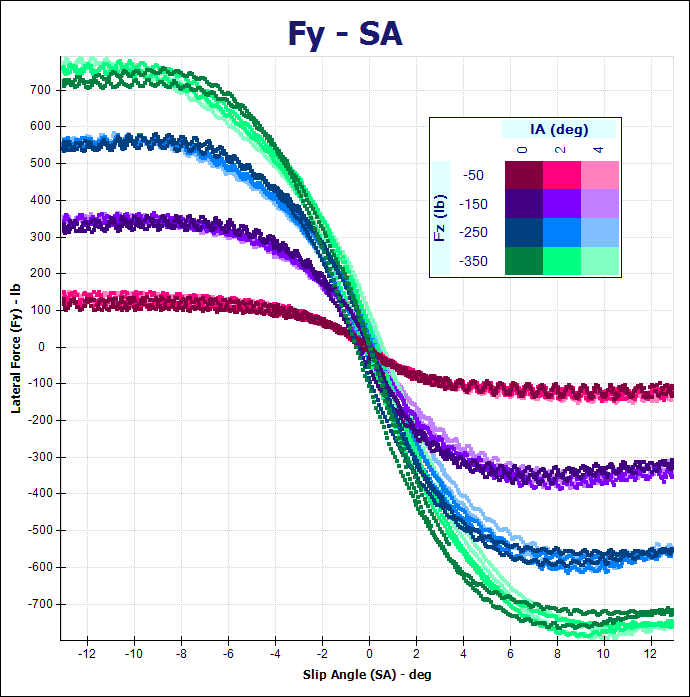
\includegraphics[width=0.9\textwidth]{UncollapsedData.png}
	\caption{Raw Data Before Collapsing}
	\label{fig:UncollapsedData}
\end{figure} 

 \begin{figure}[H]
	\centering
		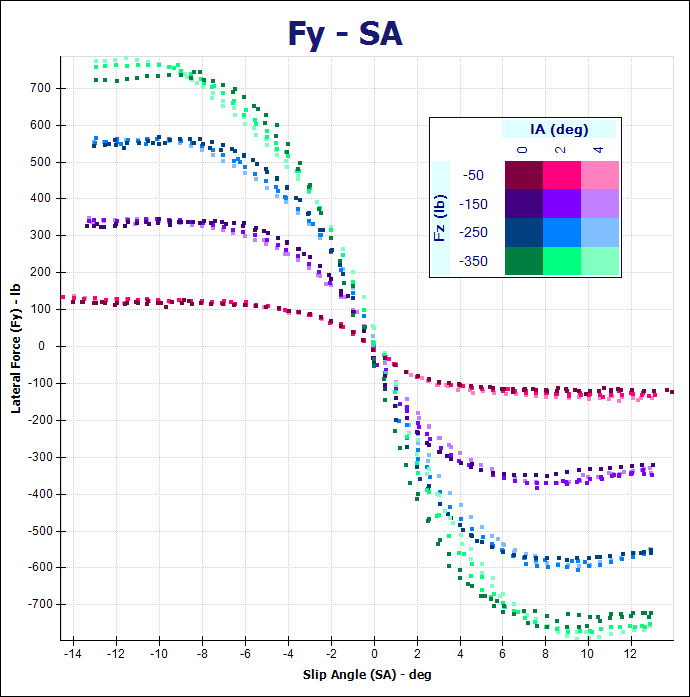
\includegraphics[width=0.9\textwidth]{CollapsedData.png}
	\caption{Collapsed Data}
	\label{fig:CollapsedData}
\end{figure} 

Now the procedure for collapsing raw data will be described. First select the raw data to be collapsed from the project tree. Then in the data entry area click on the \textsl{Collapse Data} button. This will open the data collapsing tool shown in Figure~\ref{fig:DataCollapsingTool}. 

 \begin{figure}[H]
	\centering
		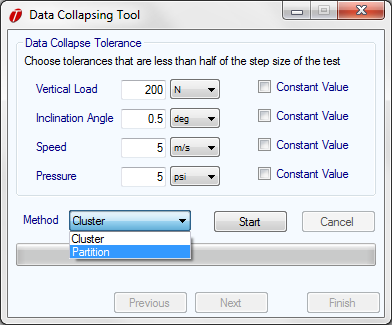
\includegraphics{DataCollapsingTool.png}
	\caption{Data Collapsing Tool}
	\label{fig:DataCollapsingTool}
\end{figure}
 
First the data is sorted into different sets depending on the test conditions. In order to do this the data collapsing tolerances should be set at less than half of the step sizes used in the tire testing. For example if a tire was tested at vertical loads of 100, 200, and 300 lbs the data tolerance should be set to at least less than 50 lbs. This will separate the different test conditions as well as sort out any irregular data. Select the constant value check box for test conditions that are kept constant throughout the test. This will increase the speed of the sorting. 

There are two sorting methods available \textsl{cluster} and \textsl{partition}. The cluster method works by creating a number of evenly spaced clusters and assigns each data point to the nearest cluster. The sizes of the initial clusters is determined by the variable tolerance. The algorithm then checks all the clusters. If the range of the cluster is too large the cluster is split if it is too small the cluster is deleted. The algorithm continues this process untill all the clusters meet the size crtieria.
The partitioning method works by assigning each data point to its own cluster. The algorithm then checks the difference between adjacent clusters if the clusters are too close they are merged. The algorithm continues until the minimum distance between clusters has met the conditions defined by the variable tolerance. 

Clicking on the \textsl{Start} button will sort the data. Once this is completed click on the \textsl{Next} button.

A list of the different sets of data will then be displayed. This is shown in Figure~\ref{fig:SortedData}. The rows of data can be sorted by value by clicking on the column headers.

It should be checked that these sets represent the data that you want to work with. Also if the data at the very beginning or end of the test was not removed with the cropping tool it can be removed here. This data will normally be at significantly different speeds or vertical loads than the rest of the data. Also if the data has a relatively low number of samples it most likely was not intended to be tested at those conditions. To remove sets of data just unselect the checkboxes next to that set. Once this is completed click on \textsl{Next}.

 \begin{figure}[H]
	\centering
		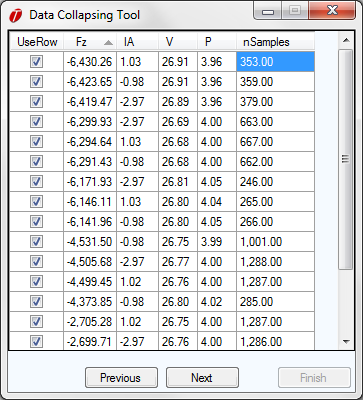
\includegraphics{SortedData.png}
	\caption{Sorted Data}
	\label{fig:SortedData}
\end{figure}

Then the discretization range over which the data will be collapsed must be selected. This is shown in Figure \ref{fig:DicretizationRange}. This determines the quantity and range of the collapsed data points that will be generated. Therefore for pure cornering data the number of steps used for the slip angle should be higher than that for the slip ratio and vice versa for the combined lateral and longitudinal data. For combined data the number of steps used should be approximately equal. 

 \begin{figure}[H]
	\centering
		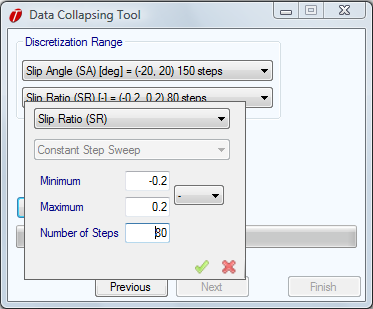
\includegraphics{DicretizationRange.png}
	\caption{Setting Discretization Range}
	\label{fig:DicretizationRange}
\end{figure}

Clicking on the \textsl{Collapse Data} button will begin the collapsing process. This will compress each set of data points that fall within each discretization step. For each step, the subsequent data points are normalized with respect to their average vertical load.   This is demonstrated in the following equations where $F_y$ is normalized with respect to the vertical load. A similar formulation is used to normalize the other output parameters (i.e.  $F_x$, $M_z$, etc�).

\begin{equation}
F_y=\frac{F_z}{F_{z0}}*F_{y0}(\alpha_0)
\end{equation}
With the normalized slip angle
\begin{equation}
\alpha_0=\frac{F_{z0}}{F_z}*\alpha
\end{equation}

Clicking on the \textsl{Finish} button will close the \textsl{Data Collapsing Tool} and return to the main OptimumTire window. A summary of the collapsed tire data will now appear in the data entry area when the tire data is selected in the project tree. The check-box labeled \textsl{Use Collapsed Data} will automatically be checked after the data is collapsed. This checkbox specifies whether the original or collapsed data will be used for graphing and fitting of tire models. This can be seen in Figure~\ref{fig:SummaryCollapsedData}.

 \begin{figure}[H]
	\centering
		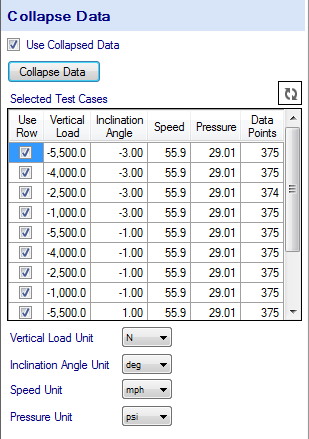
\includegraphics{SummaryCollapsedData.png}
	\caption{Summary of Collapsed Data in the Data Entry Form}
	\label{fig:SummaryCollapsedData}
\end{figure}

The summary of the collapsed data shown in Figure~\ref{fig:SummaryCollapsedData} allows the user to quickly see the data sets and the conditions of the test. The data can be sorted numerically by clicking on the column headers. The data can also be sorted by the tolerances by selecting the \textit{Sort by Tolerance} checkbox.  The checkboxes in the first column allow the user to exclude or include certain data sets from graphing and tire model fitting. Since the original raw data is still stored in OptimumTire the same data can be collapsed multiple times.

\section{Exporting Data}
\label{sec:ExportingData}
By selecting the Options-Export button at the top of the raw data entry form the tire data can be exported to an OptimumTire Raw Data File or a CSV file. After the desired format is selected a dialog box will appear. Clicking on the \textsl{Yes} button will export the cropped and collapsed tire data while clicking on the \textsl{No} button will export the raw tire data.
